% Options for packages loaded elsewhere
\PassOptionsToPackage{unicode}{hyperref}
\PassOptionsToPackage{hyphens}{url}
%
\documentclass[
  english,
  man,floatsintext]{apa7}
\usepackage{lmodern}
\usepackage{amssymb,amsmath}
\usepackage{ifxetex,ifluatex}
\ifnum 0\ifxetex 1\fi\ifluatex 1\fi=0 % if pdftex
  \usepackage[T1]{fontenc}
  \usepackage[utf8]{inputenc}
  \usepackage{textcomp} % provide euro and other symbols
\else % if luatex or xetex
  \usepackage{unicode-math}
  \defaultfontfeatures{Scale=MatchLowercase}
  \defaultfontfeatures[\rmfamily]{Ligatures=TeX,Scale=1}
\fi
% Use upquote if available, for straight quotes in verbatim environments
\IfFileExists{upquote.sty}{\usepackage{upquote}}{}
\IfFileExists{microtype.sty}{% use microtype if available
  \usepackage[]{microtype}
  \UseMicrotypeSet[protrusion]{basicmath} % disable protrusion for tt fonts
}{}
\makeatletter
\@ifundefined{KOMAClassName}{% if non-KOMA class
  \IfFileExists{parskip.sty}{%
    \usepackage{parskip}
  }{% else
    \setlength{\parindent}{0pt}
    \setlength{\parskip}{6pt plus 2pt minus 1pt}}
}{% if KOMA class
  \KOMAoptions{parskip=half}}
\makeatother
\usepackage{xcolor}
\IfFileExists{xurl.sty}{\usepackage{xurl}}{} % add URL line breaks if available
\IfFileExists{bookmark.sty}{\usepackage{bookmark}}{\usepackage{hyperref}}
\hypersetup{
  pdftitle={The Moral Dilution Effect: Irrelevant Information Influences Judgments of Moral Character},
  pdfauthor={Cillian McHugh1 \& Eric R. Igou1},
  pdflang={en},
  pdfkeywords={keywords},
  hidelinks,
  pdfcreator={LaTeX via pandoc}}
\urlstyle{same} % disable monospaced font for URLs
\usepackage{graphicx,grffile}
\makeatletter
\def\maxwidth{\ifdim\Gin@nat@width>\linewidth\linewidth\else\Gin@nat@width\fi}
\def\maxheight{\ifdim\Gin@nat@height>\textheight\textheight\else\Gin@nat@height\fi}
\makeatother
% Scale images if necessary, so that they will not overflow the page
% margins by default, and it is still possible to overwrite the defaults
% using explicit options in \includegraphics[width, height, ...]{}
\setkeys{Gin}{width=\maxwidth,height=\maxheight,keepaspectratio}
% Set default figure placement to htbp
\makeatletter
\def\fps@figure{htbp}
\makeatother
\setlength{\emergencystretch}{3em} % prevent overfull lines
\providecommand{\tightlist}{%
  \setlength{\itemsep}{0pt}\setlength{\parskip}{0pt}}
\setcounter{secnumdepth}{-\maxdimen} % remove section numbering
% Make \paragraph and \subparagraph free-standing
\ifx\paragraph\undefined\else
  \let\oldparagraph\paragraph
  \renewcommand{\paragraph}[1]{\oldparagraph{#1}\mbox{}}
\fi
\ifx\subparagraph\undefined\else
  \let\oldsubparagraph\subparagraph
  \renewcommand{\subparagraph}[1]{\oldsubparagraph{#1}\mbox{}}
\fi
% Manuscript styling
\usepackage{upgreek}
\captionsetup{font=singlespacing,justification=justified}

% Table formatting
\usepackage{longtable}
\usepackage{lscape}
% \usepackage[counterclockwise]{rotating}   % Landscape page setup for large tables
\usepackage{multirow}		% Table styling
\usepackage{tabularx}		% Control Column width
\usepackage[flushleft]{threeparttable}	% Allows for three part tables with a specified notes section
\usepackage{threeparttablex}            % Lets threeparttable work with longtable

% Create new environments so endfloat can handle them
% \newenvironment{ltable}
%   {\begin{landscape}\centering\begin{threeparttable}}
%   {\end{threeparttable}\end{landscape}}
\newenvironment{lltable}{\begin{landscape}\centering\begin{ThreePartTable}}{\end{ThreePartTable}\end{landscape}}

% Enables adjusting longtable caption width to table width
% Solution found at http://golatex.de/longtable-mit-caption-so-breit-wie-die-tabelle-t15767.html
\makeatletter
\newcommand\LastLTentrywidth{1em}
\newlength\longtablewidth
\setlength{\longtablewidth}{1in}
\newcommand{\getlongtablewidth}{\begingroup \ifcsname LT@\roman{LT@tables}\endcsname \global\longtablewidth=0pt \renewcommand{\LT@entry}[2]{\global\advance\longtablewidth by ##2\relax\gdef\LastLTentrywidth{##2}}\@nameuse{LT@\roman{LT@tables}} \fi \endgroup}

% \setlength{\parindent}{0.5in}
% \setlength{\parskip}{0pt plus 0pt minus 0pt}

% Overwrite redefinition of paragraph and subparagraph by the default LaTeX template
% See https://github.com/crsh/papaja/issues/292
\makeatletter
\renewcommand{\paragraph}{\@startsection{paragraph}{4}{\parindent}%
  {0\baselineskip \@plus 0.2ex \@minus 0.2ex}%
  {-1em}%
  {\normalfont\normalsize\bfseries\itshape\typesectitle}}

\renewcommand{\subparagraph}[1]{\@startsection{subparagraph}{5}{1em}%
  {0\baselineskip \@plus 0.2ex \@minus 0.2ex}%
  {-\z@\relax}%
  {\normalfont\normalsize\itshape\hspace{\parindent}{#1}\textit{\addperi}}{\relax}}
\makeatother

% \usepackage{etoolbox}
\makeatletter
\patchcmd{\HyOrg@maketitle}
  {\section{\normalfont\normalsize\abstractname}}
  {\section*{\normalfont\normalsize\abstractname}}
  {}{\typeout{Failed to patch abstract.}}
\patchcmd{\HyOrg@maketitle}
  {\section{\protect\normalfont{\@title}}}
  {\section*{\protect\normalfont{\@title}}}
  {}{\typeout{Failed to patch title.}}
\makeatother

\usepackage{xpatch}
\makeatletter
\xapptocmd\appendix
  {\xapptocmd\section
    {\addcontentsline{toc}{section}{\appendixname\ifoneappendix\else~\theappendix\fi\\: #1}}
    {}{\InnerPatchFailed}%
  }
{}{\PatchFailed}
\keywords{keywords\newline\indent Word count: TBC}
\usepackage{csquotes}
\raggedbottom
\ifxetex
  % Load polyglossia as late as possible: uses bidi with RTL langages (e.g. Hebrew, Arabic)
  \usepackage{polyglossia}
  \setmainlanguage[]{english}
\else
  \usepackage[shorthands=off,main=english]{babel}
\fi

\title{The Moral Dilution Effect: Irrelevant Information Influences Judgments of Moral Character}
\author{Cillian McHugh\textsuperscript{1} \& Eric R. Igou\textsuperscript{1}}
\date{}


\shorttitle{Moral Dilution}

\authornote{

Correspondence concerning this article should be addressed to Cillian McHugh, University of Limerick, Limerick, Ireland, V94 T9PX. E-mail: cillian.mchugh@.ul.ie

}

\affiliation{\vspace{0.5cm}\textsuperscript{1} University of Limerick}

\abstract{%
Across five studies we investigated the moral dilution effect
}



\begin{document}
\maketitle

Recent developments in the psychology of moral judgments propose that making a moral judgment is an act of categorization (McHugh, McGann, Igou, \& Kinsella, 2022). A corollary of this view is that moral judgments vary depending on how well a target maps onto a template of a prototypical morally relevant act/actor (Schein \& Gray, 2018)

\hypertarget{pilot-study-1}{%
\section{Pilot Study 1}\label{pilot-study-1}}

The aim of this pilot study was to develop and test materials that could be used to study the dilution effect for moral characters. We developed diagnostic and non-diagnostic character descriptions. We hypothesized that moral evaluations of the diagnostic descriptions would be more severe (more immoral) than for the non-diagnostic descriptions.

\hypertarget{pilot-study-1-method}{%
\subsection{Pilot Study 1: Method}\label{pilot-study-1-method}}

\hypertarget{pilot-1-participants-and-design}{%
\subsubsection{Pilot 1: Participants and design}\label{pilot-1-participants-and-design}}

The pilot study was a within-subjects design. The independent variable was description type with two levels, \emph{diagnostic} and \emph{non-diagnostic}. We used two dependent variables. The first dependent variable was the four item moral perception scale (MPS-4), participants rated the characters on four dimensions using 7-point bipolar scales. The dimensions and scale endpoints were: Bad-Good, Immoral-Moral, Violent-Peaceful, Merciless-Empathetic, this showed excellent reliability, \(\alpha\) = 0.93. The second dependent variable was a single item moral perception measure (MM-1) which consisted of a 100-point slider ranging from 0 = \emph{Very Immoral} to 100 = \emph{Very Moral}. Both dependent variables were taken from Walker et al.~(2021).

A total sample of 235 (89 female, 142 male, 1 non-binary, 1 prefer not to say; \emph{M}\textsubscript{age} = 36.45, min = 20, max = 72, \emph{SD} = 10.23) started the survey. Participants were recruited from MTurk.

We removed participants who failed both manipulation checks (\emph{n} = 23), leaving a total sample of 212 participants (80 female, 128 male, 1 non-binary, 1 prefer not to say; \emph{M}\textsubscript{age} = 36.63, min = 20, max = 72, \emph{SD} = 10.34).

\hypertarget{pilot-1-procedure-and-materials}{%
\subsubsection{Pilot 1: Procedure and materials}\label{pilot-1-procedure-and-materials}}

Data were collected using an online questionnaire presented with Qualtrics (www.qualtrics.com). Participants were presented with descriptions of six characters.

Moral character descriptions were developed by combining descriptions relating to three different moral foundations. These descriptions were adapted from the items of the extended character morality questionnaire (Grizzard et al., 2020). A sample description reads: \emph{Imagine a person named Sam. Throughout their life they have been known to be cruel, act unfairly, and to betray their own group}. Full text of these descriptions can be found in the supplementary materials.

We developed neutral descriptions that included information relating to physical appearance/attributes, hobbies/activities, and family information, e.g., \emph{Imagine a person named Jackie. They have red hair, play tennis four times a month, and have one older sibling and one younger sibling}.

Character descriptions did not specify the gender of the charcters, and all characters had names that could be either male or female (Sam, Robin, Francis, Alex, Jackie, Charlie). All participants read six descriptions, four moral descriptions and two neutral. Pilot Study 1 was pre-registered at \color{blue}\url{https://aspredicted.org/3VK_8FD}\color{black}.

\hypertarget{pilot-1-results}{%
\subsection{Pilot 1: Results}\label{pilot-1-results}}

The means and standard deviations for MPS-4 for each scenario are as follows:
\emph{Sam} (diagnostic),
\emph{M}\textsubscript{MPS-4} = 4.35, \emph{SD}\textsubscript{MPS-4} = 1.90,
\emph{Francis} (diagnostic),
\emph{M}\textsubscript{MPS-4} = 4.46, \emph{SD}\textsubscript{MPS-4} = 1.73,
\emph{Alex} (diagnostic),
\emph{M}\textsubscript{MPS-4} = 4.44, \emph{SD}\textsubscript{MPS-4} = 1.79,
\emph{Robin} (diagnostic),
\emph{M}\textsubscript{MPS-4} = 4.35, \emph{SD}\textsubscript{MPS-4} = 1.96,
\emph{Jackie} (non-diagnostic),
\emph{M}\textsubscript{MPS-4} = 5.40, \emph{SD}\textsubscript{MPS-4} = 1.01,
\emph{Charlie} (non-diagnostic),
\emph{M}\textsubscript{MPS-4} = 5.38, \emph{SD}\textsubscript{MPS-4} = 1.01. For the diagnostic descriptions, there was no significant variation depending on the description, \emph{F}(3,600) = 1.58, \emph{p} = .194, partial \(\eta\)\textsuperscript{2} = 0.00. For the non-diagnostic descriptions there was no significant difference in ratings depending on description, \emph{t}(211) = -0.67, \emph{p} = .506, \emph{d} = 0.05.

The means and standard deviations for MM-1 for each scenario are as follows:
\emph{Sam} (diagnostic),
\emph{M}\textsubscript{MM-1} = 55.67, \emph{SD}\textsubscript{MM-1} = 30.47;
\emph{Francis} (diagnostic),
\emph{M}\textsubscript{MM-1} = 58.22, \emph{SD}\textsubscript{MM-1} = 28.61;
\emph{Alex} (diagnostic),
\emph{M}\textsubscript{MM-1} = 56.80, \emph{SD}\textsubscript{MM-1} = 29.45;
\emph{Robin} (diagnostic),
\emph{M}\textsubscript{MM-1} = 55.49, \emph{SD}\textsubscript{MM-1} = 31.38;
\emph{Jackie} (non-diagnostic),
\emph{M}\textsubscript{MM-1} = 73.00, \emph{SD}\textsubscript{MM-1} = 14.72;
\emph{Charlie} (non-diagnostic),
\emph{M}\textsubscript{MM-1} = 72.94, \emph{SD}\textsubscript{MM-1} = 14.79. For the diagnostic descriptions, we observed significant variation depending on the description, \emph{F}(3,608) = 3.01, \emph{p} = .032, partial \(\eta\)\textsuperscript{2} = 0.001. When correcting for multiple comparisons, pairwise comparisons did not reveal significant differences between descriptions. We note that without correction, \emph{Francis} appeared to be rated as more moral than both \emph{Robin} (\emph{p} = .012), and \emph{Sam} (\emph{p} = .009). For the non-diagnostic descriptions there was no significant difference in ratings depending on description, \emph{t}(211) = -0.09, \emph{p} = .929, \emph{d} = 0.01.

We conducted a linear-mixed-effects model to test if condition influenced MPS-4 responses. Our outcome measure was MPS-4, our predictor variable was condition; we allowed intercepts and the effect of condition to vary across participants.
Overall, the model significantly predicted participants responses, and provided a better fit for the data than the baseline model, \(\chi\)\textsuperscript{2}(2) = 860.16, \emph{p} \textless{} .001. Condition was a significant predictor in the model \(b\) = -0.49, \emph{t}(211.05) = -8.54, \emph{p} \textless{} .001, with the non-diagnostic (neutral) descriptions being rated as more moral than the diagnostic (morally relevant) descriptions of immoral characters Figure~\ref{fig:pilot1bothconditionplot}.

\begin{figure}
\centering
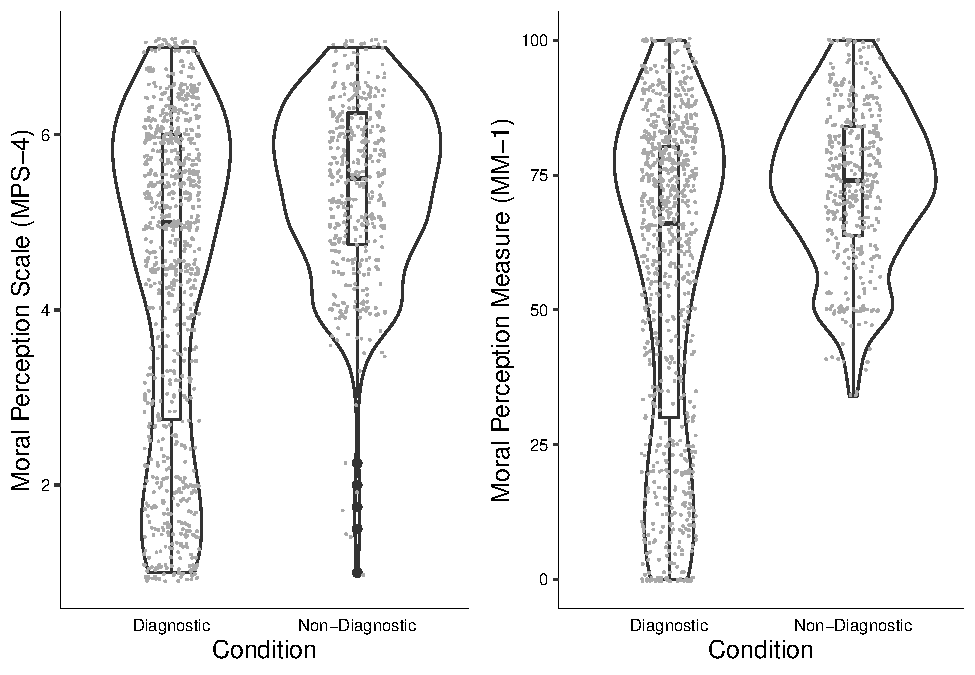
\includegraphics{moral_dilution_in_chunks_files/figure-latex/pilot1bothconditionplot-1.pdf}
\caption{\label{fig:pilot1bothconditionplot}Pilot Study 1: Differences in moral perception depending on condition}
\end{figure}

We conducted a linear-mixed-effects model to test if condition influenced MM-1 responses. Our outcome measure was MM-1, our predictor variable was condition; we allowed intercepts and the effect of condition to vary across participants. Overall, the model significantly predicted participants responses, and provided a better fit for the data than the baseline model, \(\chi\)\textsuperscript{2}(2) = 924.82, \emph{p} \textless{} .001. Condition was a significant predictor in the model \(b\) = -8.22, \emph{t}(210.98) = -8.60, \emph{p} \textless{} .001, with the non-diagnostic (neutral) descriptions being rated as more moral than the diagnostic (morally relevant) descriptions, see Figure~\ref{fig:pilot1bothconditionplot}.

\hypertarget{study-1---bad-characters}{%
\section{Study 1 - Bad Characters}\label{study-1---bad-characters}}

\hypertarget{study-1-method}{%
\subsection{Study 1: Method}\label{study-1-method}}

The aim of Study 1 is to test if the dilution effect exists in the moral domain. Participants were presented with descriptions of four characters, two descriptions will only contain diagnostic information (morally relevant information) and two will additionally contain non-diagnostic information (non morally relevant information) along with the diagnostic information. We hypothesize that moral perceptions of the diagnostic only descriptions will be more severe than for the descriptions that also contain non-diagnostic information.

\hypertarget{study-1-participants-and-design}{%
\subsubsection{Study 1: Participants and design}\label{study-1-participants-and-design}}

Study 1 was a within-subjects design. The independent variable was condition with two levels, diagnostic information only (diagnostic), and non-diagnostic information additionally included (non-diagnostic). We used the same two dependent variables as in Pilot Study 1, the four item moral perception scale (MPS-4) which showed good reliability, \(\alpha\) = 0.83, and the single item moral perception measure MM-1.

A total sample of 901 (302 female, 523 male, 0 non-binary, 5 other; 2 prefer not to say, \emph{M}\textsubscript{age} = 26.16, min = 18, max = 76, \emph{SD} = 10.14) started the survey. Participants were recruited from the student population at University of {[}BLINDED{]}.

Participants who failed both manipulation checks were removed (\emph{n} = 100), leaving a total sample of 801 participants (283 female, 496 male, 5 other, 5 prefer not to say; \emph{M}\textsubscript{age} = 26.25, min = 18, max = 76, \emph{SD} = 10.20).

\hypertarget{study-1-procedure-and-materials}{%
\subsubsection{Study 1: Procedure and materials}\label{study-1-procedure-and-materials}}

As in the pilot study, data were collected using an online questionnaire presented with Qualtrics (www.qualtrics.com). Participants were presented with four descriptions of characters (\emph{Sam}, \emph{Alex}, \emph{Francis}, \emph{Robin} from Pilot Study 1). All descriptions included diagnostic information relating to three moral foundations, e.g., \emph{Imagine a person named Robin. Throughout their life they have been known to physically hurt others, treat some people differently to others, and show lack of loyalty}. We programmed our survey to randomly present non-diagnostic information along with two of the descriptions participants read (this was done through blocking, for details on the blocks see full materials at \color{blue}\url{https://osf.io/mdnpv/?view_only=77883e3fbc3d45f1a35fe92d5318cb67}\color{black}. This meant that all participants read two descriptions containing diagnostic information only, and two descriptions that additionally included non-diagnostic information. We hypothesized that the descriptions including non-diagnostic information would be rated as less severe than the diagnostic-only descriptions. Study 1 was pre-registered at \color{blue}\url{https://aspredicted.org/DVY_QN3}\color{black}

\hypertarget{study-1-results}{%
\subsection{Study 1: Results}\label{study-1-results}}

The means and standard deviations for MPS-4 for each scenario are as follows:
\emph{Sam},
\emph{M}\textsubscript{MPS-4} = 2.55, \emph{SD}\textsubscript{MPS-4} = 0.86,
\emph{Francis},
\emph{M}\textsubscript{MPS-4} = 3.05, \emph{SD}\textsubscript{MPS-4} = 0.97,
\emph{Alex},
\emph{M}\textsubscript{MPS-4} = 2.32, \emph{SD}\textsubscript{MPS-4} = 0.88,
\emph{Robin},
\emph{M}\textsubscript{MPS-4} = 2.13, \emph{SD}\textsubscript{MPS-4} = 0.91. There was significant variation depending on the description, \emph{F}(3,2280) = 297.82, \emph{p} \textless{} .001, partial \(\eta\)\textsuperscript{2} = 0.13. \emph{Francis} appeared to be rated as more moral than each of the other characters (all \emph{p}s \textless{} .001), while \emph{Robin} was rated as less moral than each of the other characters (all \emph{p}s \textless{} .001), while \emph{Sam} was rated more favorably than \emph{Alex} (\emph{p} \textless{} .001).

The means and standard deviations for MM-1 for each scenario are as follows:
\emph{Sam},
\emph{M}\textsubscript{MM-1} = 23.94, \emph{SD}\textsubscript{MM-1} = 16.18;
\emph{Francis},
\emph{M}\textsubscript{MM-1} = 30.12, \emph{SD}\textsubscript{MM-1} = 17.86;
\emph{Alex},
\emph{M}\textsubscript{MM-1} = 20.55, \emph{SD}\textsubscript{MM-1} = 16.65;
\emph{Robin},
\emph{M}\textsubscript{MM-1} = 20.60, \emph{SD}\textsubscript{MM-1} = 17.06. There was significant variation depending on the description, \emph{F}(3,2253) = 154.08, \emph{p} \textless{} .001, partial \(\eta\)\textsuperscript{2} = 0.05. \emph{Francis} was rated more favorably than all other characters (\emph{p} \textless{} .001), \emph{Sam} was the next most favorably rated character, rated significantly more favorably than both \emph{Alex} and \emph{Robin} (\emph{p}s \textless{} .001), there was no difference between \emph{Alex} and \emph{Robin} (\emph{p} = = .953).

We conducted a linear-mixed-effects model to test if condition influenced MPS-4 responses. Our outcome measure was MPS-4, our predictor variable was condition; we allowed intercepts and the effect of condition to vary across participants, and scenario was also included in the model.
Overall, the model significantly predicted participants responses, and provided a better fit for the data than the baseline model, \(\chi\)\textsuperscript{2}(8) = 816.91, \emph{p} \textless{} .001. Condition significantly influenced responses to the MPS-4, \emph{F}(1, 799.42) = 51.47, \emph{p} \textless{} .001; and was a significant predictor in the model when controlling for scenario, \(b\) = -0.08, \emph{t}(799.42) = -7.17, \emph{p} \textless{} .001, with the diagnostic descriptions being rated as more immoral than the non-diagnostic descriptions Figure~\ref{fig:S1bothconditionplot}.

\begin{figure}
\centering
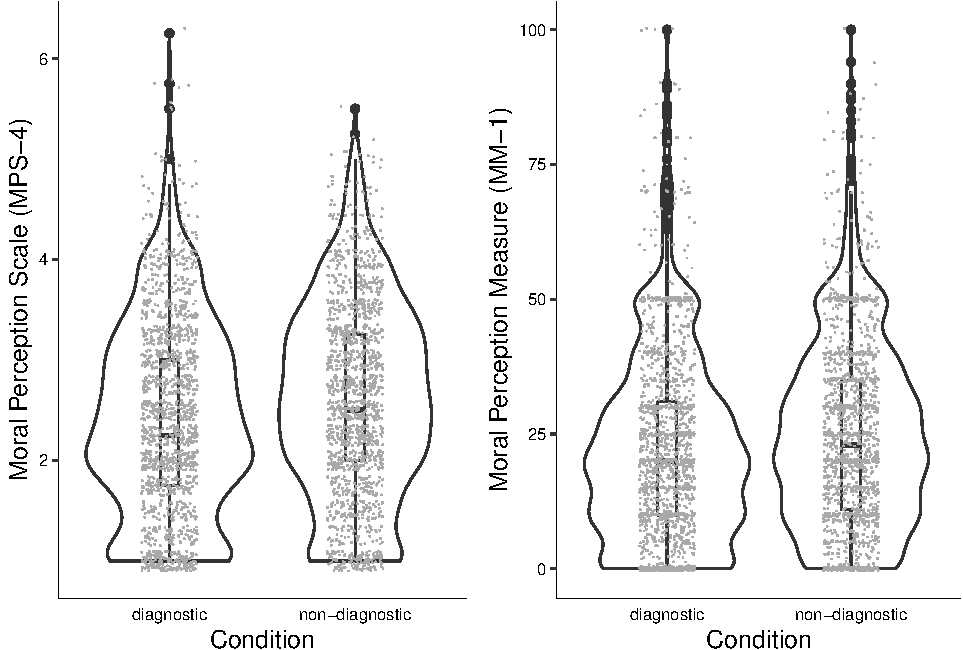
\includegraphics{moral_dilution_in_chunks_files/figure-latex/S1bothconditionplot-1.pdf}
\caption{\label{fig:S1bothconditionplot}Study 1: Differences in moral perception depending on condition}
\end{figure}

We conducted a linear-mixed-effects model to test if condition influenced MM-1 responses. Our outcome measure was MM-1, our predictor variable was condition; we allowed intercepts and the effect of condition to vary across participants. Overall, the model significantly predicted participants responses, and provided a better fit for the data than the baseline model, \(\chi\)\textsuperscript{2}(8) = 475.52, \emph{p} \textless{} .001. Condition significantly predicted MM-1 responses \emph{F}(1, 799.71) = 44.39, \emph{p} \textless{} .001, and when controlling for scenario was a significant predictor in the model \(b\) = -1.22, \emph{t}(799.71) = -6.66, \emph{p} \textless{} .001, with the diagnostic descriptions being rated as more immoral than the non-diagnostic descriptions Figure~\ref{fig:S1bothconditionplot}.

In the supplementary analyses we report the effect of condition on moral perception for each description individually.

\hypertarget{pilot-study-2}{%
\section{Pilot Study 2}\label{pilot-study-2}}

Study 1 showed the moral dilution effect for judgments of \emph{bad} characters. The aim of this pilot study was to develop and test materials that may be used to study the moral dilution effect for judgments of morally \emph{good} characters. As with Pilot Study 1, we developed diagnostic and non-diagnostic descriptions. We hypothesized that evaluations of the diagnostic descriptions would be more extreme (more moral) than for the non-diagnostic descriptions

\hypertarget{pilot-study-2-method}{%
\subsection{Pilot Study 2: Method}\label{pilot-study-2-method}}

\hypertarget{pilot-2-participants-and-design}{%
\subsubsection{Pilot 2: Participants and design}\label{pilot-2-participants-and-design}}

The pilot study was a within-subjects design. The independent variable was description type with two levels, \emph{diagnostic} and \emph{non-diagnostic}. We used the same two dependent variables as in previous studies, the four item moral perception scale (MPS-4, \(\alpha\) = 0.84), and the single item moral perception measure (MM-1).

A total sample of 245 (70 female, 175 male, 0 non-binary, 0 prefer not to say; \emph{M}\textsubscript{age} = 36.69, min = 18, max = 71, \emph{SD} = 9.57) started the survey. Participants were recruited from MTurk.

We removed participants who failed both manipulation checks (\emph{n} = 30), leaving a total sample of 215 participants (63 female, 152 male, 0 non-binary, 0 prefer not to say; \emph{M}\textsubscript{age} = 36.59, min = 18, max = 71, \emph{SD} = 9.59).

\hypertarget{pilot-2-procedure-and-materials}{%
\subsubsection{Pilot 2: Procedure and materials}\label{pilot-2-procedure-and-materials}}

Data were collected using an online questionnaire presented with Qualtrics (www.qualtrics.com). Participants were presented with descriptions of six characters.

Moral character descriptions were developed by combining descriptions relating to three different moral foundations, focusing on upholding the moral foundations (rather than transgressions as in previous studies). A sample description reads: \emph{Imagine a person named Sam. Throughout their life they have been known to always help and care for others, treat everyone fairly and equally, and show a strong sense of loyalty to others.}. Full text of these descriptions can be found in the supplementary materials.

We developed neutral descriptions that included information relating to physical appearance/attributes, hobbies/activities, and a color preference, e.g., \emph{Imagine a person named Charlie. They have blue eyes, drink coffee in the morning, and their favourite colour is green}.

We used the same gender ambiguous names, and we did not specify the gender of the characters. Pilot Study 2 was pre-registered at \color{blue}\url{https://aspredicted.org/W52_VPX}\color{black}.

\hypertarget{pilot-2-results}{%
\subsection{Pilot 2: Results}\label{pilot-2-results}}

The means and standard deviations for MPS-4 for each scenario are as follows:
\emph{Sam} (diagnostic/moral),
\emph{M}\textsubscript{MPS-4} = 6.01, \emph{SD}\textsubscript{MPS-4} = 0.91,
\emph{Francis} (diagnostic/moral),
\emph{M}\textsubscript{MPS-4} = 5.89, \emph{SD}\textsubscript{MPS-4} = 0.95,
\emph{Alex} (diagnostic/moral),
\emph{M}\textsubscript{MPS-4} = 5.94, \emph{SD}\textsubscript{MPS-4} = 0.94,
\emph{Robin} (diagnostic/moral),
\emph{M}\textsubscript{MPS-4} = 5.93, \emph{SD}\textsubscript{MPS-4} = 0.92,
\emph{Jackie} (non-diagnostic/neutral),
\emph{M}\textsubscript{MPS-4} = 5.60, \emph{SD}\textsubscript{MPS-4} = 0.99,
\emph{Charlie} (non-diagnostic/neutral),
\emph{M}\textsubscript{MPS-4} = 5.53, \emph{SD}\textsubscript{MPS-4} = 1.08. For the diagnostic descriptions, there was significant variation depending on the description, \emph{F}(3,613) = 2.91, \emph{p} = .036, partial \(\eta\)\textsuperscript{2} = 0.00, \emph{Sam} was viewed significantly more favorably than \emph{Francis} (\emph{p} = .040). For the non-diagnostic descriptions there was no significant difference in ratings depending on description, \emph{t}(214) = -1.79, \emph{p} = .075, \emph{d} = 0.12.

The means and standard deviations for MM-1 for each scenario are as follows:
\emph{Sam} (diagnostic/moral),
\emph{M}\textsubscript{MM-1} = 79.85, \emph{SD}\textsubscript{MM-1} = 15.44;
\emph{Francis} (diagnostic/moral),
\emph{M}\textsubscript{MM-1} = 78.30, \emph{SD}\textsubscript{MM-1} = 15.84;
\emph{Alex} (diagnostic/moral),
\emph{M}\textsubscript{MM-1} = 79.78, \emph{SD}\textsubscript{MM-1} = 15.71;
\emph{Robin} (diagnostic/moral),
\emph{M}\textsubscript{MM-1} = 79.46, \emph{SD}\textsubscript{MM-1} = 15.41;
\emph{Jackie} (non-diagnostic/neutral),
\emph{M}\textsubscript{MM-1} = 73.44, \emph{SD}\textsubscript{MM-1} = 15.83;
\emph{Charlie} (non-diagnostic/neutral),
\emph{M}\textsubscript{MM-1} = 73.07, \emph{SD}\textsubscript{MM-1} = 16.22. For the diagnostic descriptions, we observed no significant variation depending on the description, \emph{F}(3,594) = 1.45, \emph{p} = .231, partial \(\eta\)\textsuperscript{2} = 0.002. For the non-diagnostic descriptions there was no significant difference in ratings depending on description, \emph{t}(214) = -0.60, \emph{p} = .552, \emph{d} = 0.04.

We conducted a linear-mixed-effects model to test if condition influenced MPS-4 responses. Our outcome measure was MPS-4, our predictor variable was condition; we allowed intercepts and the effect of condition to vary across participants.
Overall, the model significantly predicted participants responses, and provided a better fit for the data than the baseline model, \(\chi\)\textsuperscript{2}(2) = 475.42, \emph{p} \textless{} .001. Condition was a significant predictor in the model \(b\) = 0.19, \emph{t}(214.35) = 6.53, \emph{p} \textless{} .001, with the diagnostic descriptions being rated as more moral than the non-diagnostic descriptions of immoral characters Figure~\ref{fig:pilot2bothconditionplot}.

\begin{figure}
\centering
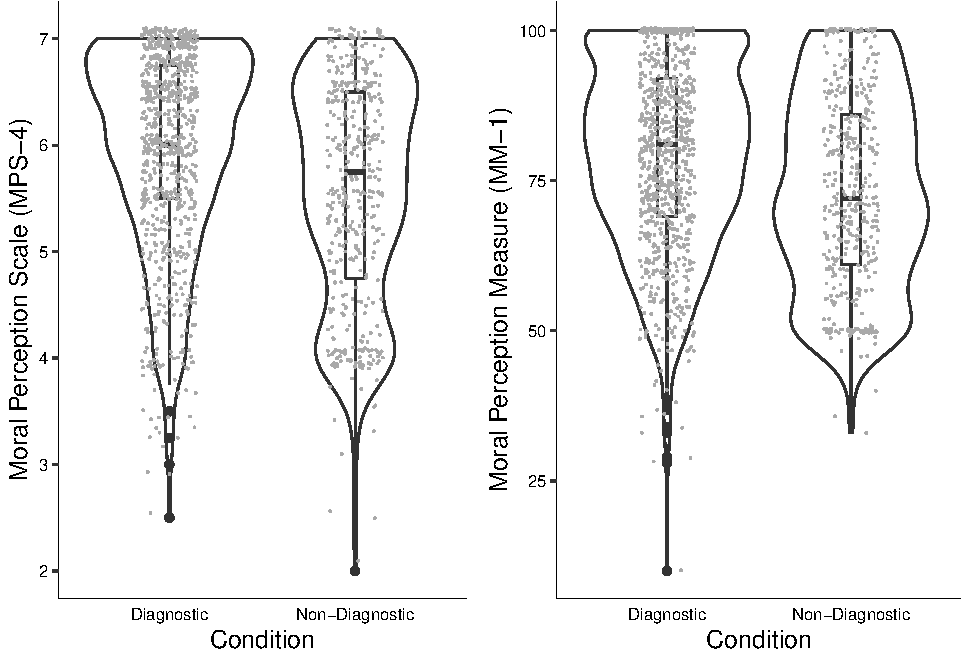
\includegraphics{moral_dilution_in_chunks_files/figure-latex/pilot2bothconditionplot-1.pdf}
\caption{\label{fig:pilot2bothconditionplot}Pilot Study 2: Differences in moral perception depending on condition}
\end{figure}

We conducted a linear-mixed-effects model to test if condition influenced MM-1 responses. Our outcome measure was MM-1, our predictor variable was condition; we allowed intercepts and the effect of condition to vary across participants. Overall, the model significantly predicted participants responses, and provided a better fit for the data than the baseline model, \(\chi\)\textsuperscript{2}(2) = 324.13, \emph{p} \textless{} .001. Condition was a significant predictor in the model \(b\) = 3.04, \emph{t}(214.90) = 6.02, \emph{p} \textless{} .001, with the diagnostic descriptions being rated as more moral than the non-diagnostic descriptions, see Figure~\ref{fig:pilot2bothconditionplot}.

\hypertarget{study-2---good-characters}{%
\section{Study 2 - Good Characters}\label{study-2---good-characters}}

The aim of Study 2 is to test if the dilution effect exists in the moral domain for judgments of morally \emph{good} characters. Participants were presented with descriptions of four characters, two descriptions contain diagnostic information only (morally relevant information) and two will additionally contain non-diagnostic information (non morally relevant information) along with the diagnostic information. We hypothesize that moral perceptions of the diagnostic only descriptions will be more extreme (more moral) than for the descriptions that also contain non-diagnostic information.

\hypertarget{study-2-method}{%
\subsection{Study 2: Method}\label{study-2-method}}

\hypertarget{study-2-participants-and-design}{%
\subsubsection{Study 2: Participants and design}\label{study-2-participants-and-design}}

Study 2 was a within-subjects design. The independent variable was condition with two levels, diagnostic and non-diagnostic. We used the same two dependent variables as in previous studies, the four item moral perception scale (MPS-4, \(\alpha\) = 0.85), and the single item moral perception measure MM-1.

A total sample of 1068 (418 female, 557 male, 13 non-binary, 2 other; 4 prefer not to say, \emph{M}\textsubscript{age} = 29.04, min = 18, max = 74, \emph{SD} = 10.66) started the survey. Participants were recruited from the student population at University of {[}BLINDED{]}.

Participants who failed both manipulation checks were removed (\emph{n} = 248), leaving a total sample of 820 participants (337 female, 466 male, 2 other, 2 prefer not to say; \emph{M}\textsubscript{age} = 29.03, min = 18, max = 74, \emph{SD} = 10.92).

The majority of participants were from the student body: \emph{n} = 533, (female = 370, male = 147, non-binary/other = 14, prefer not to say 3, \emph{M\textsubscript{age}} = 25.50, \emph{SD} = 9.60).

In order to reach our pre-registered target sample size we recruited additional participants from MTurk: \emph{n} = 287, (female = 96, male = 190, non-binary/other = 1, prefer not to say 1, \emph{M\textsubscript{age}} = 35.70, \emph{SD} = 10.10). Participants from MTurk were paid \$0.40 for their participation.

\hypertarget{study-2-procedure-and-materials}{%
\subsubsection{Study 2: Procedure and materials}\label{study-2-procedure-and-materials}}

Again, data were collected using an online questionnaire presented with Qualtrics (www.qualtrics.com). Participants were presented with four descriptions of characters (\emph{Sam}, \emph{Alex}, \emph{Francis}, \emph{Robin} from Pilot Study 2). All descriptions included diagnostic information relating to three moral foundations, e.g., \emph{Imagine a person named Alex. Throughout their life they have been known to protect and provide shelter to the weak and vulnerable, uphold the rights of others, and show respect for authority}. For each participant, two descriptions additionally included non-diagnostic information (this was randomized through blocking, see \color{blue}\url{https://osf.io/mdnpv/?view_only=77883e3fbc3d45f1a35fe92d5318cb67}\color{black}. Study 1 was pre-registered at \color{blue}\url{https://aspredicted.org/NX2_HN6}\color{black}

\hypertarget{study-2-results}{%
\subsection{Study 2: Results}\label{study-2-results}}

The means and standard deviations for MPS-4 for each scenario are as follows:
\emph{Sam},
\emph{M}\textsubscript{MPS-4} = 6.12, \emph{SD}\textsubscript{MPS-4} = 0.97,
\emph{Francis},
\emph{M}\textsubscript{MPS-4} = 5.86, \emph{SD}\textsubscript{MPS-4} = 1.07,
\emph{Alex},
\emph{M}\textsubscript{MPS-4} = 6.13, \emph{SD}\textsubscript{MPS-4} = 0.99,
\emph{Robin},
\emph{M}\textsubscript{MPS-4} = 6.10, \emph{SD}\textsubscript{MPS-4} = 0.99. There was significant variation depending on the description, \emph{F}(3,2356) = 54.47, \emph{p} \textless{} .001, partial \(\eta\)\textsuperscript{2} = 0.01. \emph{Francis} appeared to be rated as less moral than each of the other characters (all \emph{p}s \textless{} .001).

The means and standard deviations for MM-1 for each scenario are as follows:
\emph{Sam} (diagnostic/moral),
\emph{M}\textsubscript{MM-1} = 84.60, \emph{SD}\textsubscript{MM-1} = 14.47;
\emph{Francis} (diagnostic/moral),
\emph{M}\textsubscript{MM-1} = 82.05, \emph{SD}\textsubscript{MM-1} = 15.24;
\emph{Alex} (diagnostic/moral),
\emph{M}\textsubscript{MM-1} = 85.02, \emph{SD}\textsubscript{MM-1} = 15.01;
\emph{Robin} (diagnostic/moral),
\emph{M}\textsubscript{MM-1} = 84.95, \emph{SD}\textsubscript{MM-1} = 13.94. There was significant variation depending on the description, \emph{F}(3,2387) = 24.20, \emph{p} \textless{} .001, partial \(\eta\)\textsuperscript{2} = 0.007. \emph{Francis} was rated less favorably than all other characters (all \emph{p}s \textless{} .001).

We conducted a linear-mixed-effects model to test if condition influenced MPS-4 responses. Our outcome measure was MPS-4, our predictor variable was condition; we allowed intercepts and the effect of condition to vary across participants, and scenario was also included in the model.
Overall, the model significantly predicted participants responses, and provided a better fit for the data than the baseline model, \(\chi\)\textsuperscript{2}(8) = 160.00, \emph{p} \textless{} .001. Condition did not influence responses to the MPS-4, \emph{F}(1, 838.12) = 0.24, \emph{p} = .624; and was not a significant predictor in the model when controlling for scenario, \(b\) = 0.00, \emph{t}(838) = 0.49, \emph{p} = .624, see Figure~\ref{fig:S2bothconditionplot}.

\begin{figure}
\centering
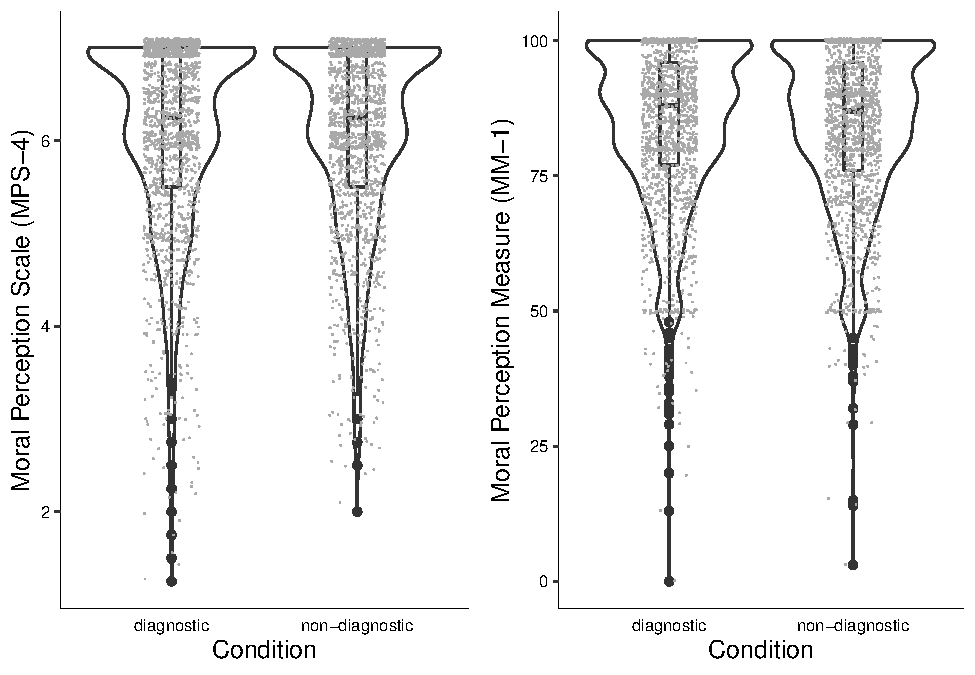
\includegraphics{moral_dilution_in_chunks_files/figure-latex/S2bothconditionplot-1.pdf}
\caption{\label{fig:S2bothconditionplot}Study 2: Differences in moral perception depending on condition}
\end{figure}

We conducted a linear-mixed-effects model to test if condition influenced MM-1 responses. Our outcome measure was MM-1, our predictor variable was condition; we allowed intercepts and the effect of condition to vary across participants. Overall, the model significantly predicted participants responses, and provided a better fit for the data than the baseline model, \(\chi\)\textsuperscript{2}(8) = 75.69, \emph{p} \textless{} .001. Condition did not influence MM-1 responses \emph{F}(1, 2453) = 1.23, \emph{p} = .267, and was not a significant predictor in the model \(b\) = 0.16, \emph{t}(2453) = 1.11, \emph{p} = .267, see Figure~\ref{fig:S2bothconditionplot}.

In the supplementary analyses we report the effect of condition on moral perception for each description individually.

\hypertarget{study-3---good-and-bad-characters}{%
\section{Study 3 - Good and Bad Characters}\label{study-3---good-and-bad-characters}}

In Study 1 we found evidence for the moral dilution effect for judgments of \emph{bad} moral characters. In Study 2 we failed replicate this effect for judgments of \emph{good} moral characters. The aim of Study 3 was to test if valence (good vs.~bad) moderates the moral dilution effect. We hypothesized that valence (good vs bad) would interact with condition in producing a dilution effect, such that the dilution effect would be observed for bad characters but not for good characters. Study 3 was pre-registered at \color{blue}\url{https://aspredicted.org/QDF_XT1}\color{black}.

\hypertarget{study-3-method}{%
\subsection{Study 3: Method}\label{study-3-method}}

\hypertarget{study-3-participants-and-design}{%
\subsubsection{Study 3: Participants and design}\label{study-3-participants-and-design}}

Study 3 was a 2 \(\times\) 2 within-subjects factorial design. The first independent variable was condition with two levels, diagnostic and non-diagnostic. The second independent variable was valence of character description, with two levels morally good and morally bad. We used the same two dependent variables as in previous studies, the four item moral perception scale (MPS-4, \(\alpha\) = 0.94), and the single item moral perception measure MM-1.

A total sample of 1095 (700 female, 386 male, 2 non-binary, 0 other; 2 prefer not to say, \emph{M}\textsubscript{age} = 36.42, min = 19, max = 77, \emph{SD} = 10.65) started the survey. Participants were recruited from MTurk and paid \$0.40 for their participation.

Participants who failed both manipulation checks were removed (\emph{n} = 221), leaving a total sample of 874 participants (550 female, 320 male, 0 other, 0 prefer not to say; \emph{M}\textsubscript{age} = 36.37, min = 19, max = 77, \emph{SD} = 10.72).

\hypertarget{study-3-procedure-and-materials}{%
\subsubsection{Study 3: Procedure and materials}\label{study-3-procedure-and-materials}}

Again, data were collected using an online questionnaire presented with Qualtrics (www.qualtrics.com). Participants were presented with four descriptions of characters taken from Studies 1 and 2. To ensure consistency across character judgments, we selected descriptions that related to the same moral foundations (care, fairness, and loyalty). We used the same four character names as in previous studies. The \emph{good} characters were \emph{Sam} and \emph{Robin}, and the \emph{bad} characters were \emph{Francis} and \emph{Alex}, e.g., \emph{Imagine a person named Robin. Throughout their life they have been known to show compassion and empathy for others, act with a sense of fairness and justice, and, never to break their word.} or, \emph{Imagine a person named Alex. Throughout their life they have been known to be cruel, act unfairly, and to betray their own group.} Full descriptions for each character are in the supplementary materials. One description for each the \emph{good} and \emph{bad} characters was randomly assigned to include non-diagnostic information for each participant thus all participants were exposed to all conditions (see \color{blue}\url{https://osf.io/mdnpv/?view_only=77883e3fbc3d45f1a35fe92d5318cb67}\color{black} for details of the randomization blocks). Study 3 was pre-registered at \color{blue}\url{https://aspredicted.org/QDF_XT1}\color{black}

\hypertarget{study-3-results}{%
\subsection{Study 3: Results}\label{study-3-results}}

The means and standard deviations for MPS-4 for each scenario are as follows:
\emph{Sam} (good),
\emph{M}\textsubscript{MPS-4} = 5.90, \emph{SD}\textsubscript{MPS-4} = 1.03,
\emph{Francis} (bad),
\emph{M}\textsubscript{MPS-4} = 4.07, \emph{SD}\textsubscript{MPS-4} = 2.07,
\emph{Alex} (bad),
\emph{M}\textsubscript{MPS-4} = 4.03, \emph{SD}\textsubscript{MPS-4} = 2.03,
\emph{Robin} (good),
\emph{M}\textsubscript{MPS-4} = 5.85, \emph{SD}\textsubscript{MPS-4} = 1.05. There was significant variation depending on the description, \emph{F}(1,1080) = 442.71, \emph{p} \textless{} .001, partial \(\eta\)\textsuperscript{2} = 0.24. Both the \emph{good} characters (\emph{Robin} and \emph{Sam}) were rated significantly more favorably than both the \emph{bad} characters (\emph{Alex} and \emph{Francis}; all \emph{p}s \textless{} .001). There were no differences between \emph{Robin} and \emph{Sam} (\emph{good}: \emph{p} = .366) or between \emph{Alex} and \emph{Francis} (\emph{bad}; (\emph{p} = .648)).

The means and standard deviations for MM-1 for each scenario are as follows:
\emph{Sam} (good),
\emph{M}\textsubscript{MM-1} = 81.01, \emph{SD}\textsubscript{MM-1} = 15.23;
\emph{Francis} (bad),
\emph{M}\textsubscript{MM-1} = 51.49, \emph{SD}\textsubscript{MM-1} = 33.18;
\emph{Alex} (bad),
\emph{M}\textsubscript{MM-1} = 50.89, \emph{SD}\textsubscript{MM-1} = 32.14;
\emph{Robin} (good),
\emph{M}\textsubscript{MM-1} = 80.81, \emph{SD}\textsubscript{MM-1} = 15.16. There was significant variation depending on the description, \emph{F}(1,1080) = 458.92, \emph{p} \textless{} .001, partial \(\eta\)\textsuperscript{2} = 0.254. Again, the \emph{good} characters (\emph{Robin} and \emph{Sam}) were rated significantly more favorably than the \emph{bad} characters (\emph{Alex} and \emph{Francis}; all \emph{p}s \textless{} .001). There were no differences between \emph{Robin} and \emph{Sam} (\emph{good}: \emph{p} = .776) or between \emph{Alex} and \emph{Francis} (\emph{bad}; (\emph{p} = .683)).

We conducted a linear-mixed-effects model to test if our predictors influenced MPS-4 responses. Our outcome measure was MPS-4, our predictor variables were condition and valence; we allowed intercepts and the effects of condition and valence to vary across participants.
Overall, the model significantly predicted participants responses, and provided a better fit for the data than the baseline model,
\(\chi\)\textsuperscript{2}(5) = 3,420.34, \emph{p} \textless{} .001.
As expected, on its own, condition did not influence responses to the MPS-4
, \emph{F}(1, 1746) = 0.01, \emph{p} = .937
; valence significantly predicted responses,
, \emph{F}(1, 1746) = 587.37, \emph{p} \textless{} .001
; and there was a significant condition \(\times\) valence interaction,
, \emph{F}(1, 1746) = 9.13, \emph{p} = .003.
and was not a significant predictor in the model when controlling for scenario, \(b\) = 0.00, \emph{t}(1,746.00) = -0.08, \emph{p} = .937.

We conducted a linear-mixed-effects model to test if our predictors influenced MM-1 responses. The model was the same as the previous model, with a change to the outcome measure, our outcome measure for this model was MM-1. As above, our predictor variables were condition and valence; we allowed intercepts and the effects of condition and valence to vary across participants.
Overall, the model significantly predicted participants responses, and provided a better fit for the data than the baseline model,
\(\chi\)\textsuperscript{2}(5) = 3,441.43, \emph{p} \textless{} .001.
As expected, on its own, condition did not influence responses to the MPS-4
, \emph{F}(1, 1746) = 0.03, \emph{p} = .852
; valence significantly predicted responses,
, \emph{F}(1, 1746) = 638.14, \emph{p} \textless{} .001
; and there was a significant condition \(\times\) valence interaction,
, \emph{F}(1, 1746) = 17.23, \emph{p} \textless{} .001.
and was not a significant predictor in the model when controlling for scenario, \(b\) = -0.03, \emph{t}(1,746.00) = -0.19, \emph{p} = .852.

\hypertarget{differences-in-the-bad-descriptions}{%
\subsection{\texorpdfstring{Differences in the \emph{Bad} Descriptions}{Differences in the Bad Descriptions}}\label{differences-in-the-bad-descriptions}}

To interpret the interaction effect, we conducted separate analyses for the Good and Bad descriptions.

We conducted a linear-mixed-effects model to test if condition influenced MPS-4 responses. Our outcome measure was MPS-4, our predictor variable was condition; we allowed intercepts and the effect of condition to vary across participants. Overall, the model did not significantly predict participants responses, or provide a better fit for the data than the baseline model, \(\chi\)\textsuperscript{2}(3) = 5.40, \emph{p} = .145. Condition did not significantly influence MPS-4 responses \emph{F}(1, 872.00) = 3.54, \emph{p} = .060, and was not a significant predictor in the model \(b\) = -0.03, \emph{t}(872.00) = -1.88, \emph{p} = .060, see Figure~\ref{fig:S3bothconditionplot}.

We conducted a linear-mixed-effects model to test if condition influenced MM-1 responses. Our outcome measure was MM-1, our predictor variable was condition; we allowed intercepts and the effect of condition to vary across participants. Overall, the model significantly predicted participants responses, and provided a better fit for the data than the baseline model, \(\chi\)\textsuperscript{2}(3) = 8.67, \emph{p} = .034. Condition significantly influenced MM-1 responses \emph{F}(1, 872.00) = 7.01, \emph{p} = .008, and was a significant predictor in the model \(b\) = -0.69, \emph{t}(872.00) = -2.65, \emph{p} = .008, see Figure~\ref{fig:S3bothconditionplot}.

\hypertarget{differences-in-the-good-descriptions}{%
\subsection{\texorpdfstring{Differences in the \emph{Good} Descriptions}{Differences in the Good Descriptions}}\label{differences-in-the-good-descriptions}}

To interpret the interaction effect, we conducted separate analyses for the Good and Bad descriptions.

We conducted a linear-mixed-effects model to test if condition influenced MPS-4 responses. Our outcome measure was MPS-4, our predictor variable was condition; we allowed intercepts and the effect of condition to vary across participants. Overall, the model significantly predicted participants responses, and provided a better fit for the data than the baseline model, \(\chi\)\textsuperscript{2}(3) = 13.66, \emph{p} = .003. Condition significantly influenced MPS-4 responses \emph{F}(1, 872.00) = 6.82, \emph{p} = .009, and was a significant predictor in the model \(b\) = 0.03, \emph{t}(872.00) = 2.61, \emph{p} = .009, see Figure~\ref{fig:S3bothconditionplot}.

\begin{figure}
\centering
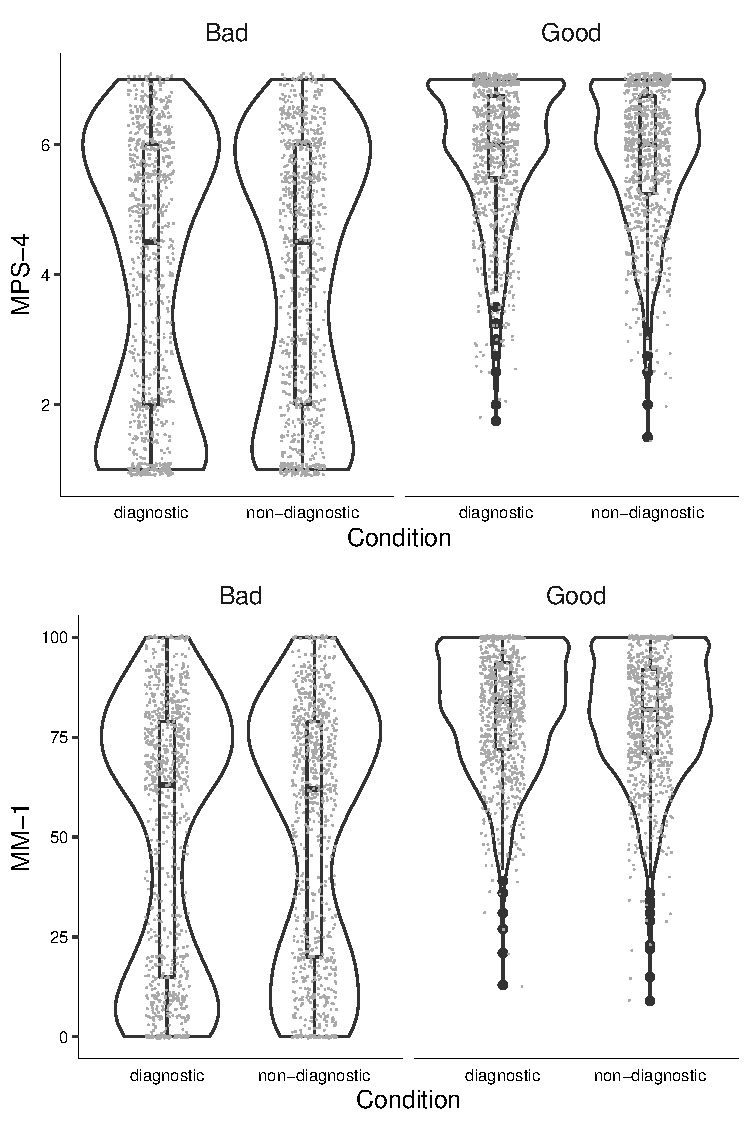
\includegraphics{moral_dilution_in_chunks_files/figure-latex/S3bothconditionplot-1.pdf}
\caption{\label{fig:S3bothconditionplot}Study 3: Differences in moral perception depending on condition}
\end{figure}

We conducted a linear-mixed-effects model to test if condition influenced MM-1 responses. Our outcome measure was MM-1, our predictor variable was condition; we allowed intercepts and the effect of condition to vary across participants. Overall, the model significantly predicted participants responses, and provided a better fit for the data than the baseline model, \(\chi\)\textsuperscript{2}(1) = 11.97, \emph{p} \textless{} .001. Condition significantly influenced MM-1 responses \emph{F}(1, 873) = 12.04, \emph{p} \textless{} .001, and was a significant predictor in the model \(b\) = 0.63, \emph{t}(873) = 3.47, \emph{p} \textless{} .001, see Figure~\ref{fig:S3bothconditionplot}.

In the supplementary analyses we report the effect of condition on moral perception for each description individually.

The aim of Study 3 was to test if the moral dilution effect was moderated by valence of description. Based on the results of Studies 1 and 2 we hypothesized that a dilution effect would be observed for judgments of \emph{bad} characters, but not for judgments of \emph{good} characters. Interestingly, in Study 2 we found a dilution effect for \emph{good} characters across both measures, however we only found a dilution effect for \emph{bad} characters when using the single item measure of moral perception.

\hypertarget{study-4---good-characters}{%
\section{Study 4 - Good Characters}\label{study-4---good-characters}}

Following the divergent results for morally good characters between Studies 2 and 3, Study 4 was an attempted replication of Study 2.

\hypertarget{study-4-method}{%
\subsection{Study 4: Method}\label{study-4-method}}

\hypertarget{study-4-participants-and-design}{%
\subsubsection{Study 4: Participants and design}\label{study-4-participants-and-design}}

The design, materials, and procedure for Study 4 were the same as for Study 2, the only change from Study 2 was that all participants in Study 4 were recruited from MTurk. Study 4 was a within-subjects design. The independent variable was condition with two levels, diagnostic and non-diagnostic. We used the same two dependent variables as in previous studies, the four item moral perception scale (MPS-4, \(\alpha\) = 0.81), and the single item moral perception measure MM-1.

A total sample of 1118 (642 female, 445 male, 2 non-binary, 3 other; 1 prefer not to say, \emph{M}\textsubscript{age} = 37.44, min = 19, max = 84, \emph{SD} = 11.08) started the survey. Participants were recruited from MTurk and paid \$0.40 for their participation.

Participants who failed both manipulation checks were removed (\emph{n} = 262), leaving a total sample of 856 participants (507 female, 347 male, 0 other, 0 prefer not to say; \emph{M}\textsubscript{age} = 37.12, min = 19, max = 84, \emph{SD} = 11.04).

\hypertarget{study-4-procedure-and-materials}{%
\subsubsection{Study 4: Procedure and materials}\label{study-4-procedure-and-materials}}

All materials and procedures were the same as in Study 2.

\hypertarget{study-4-results}{%
\subsection{Study 4: Results}\label{study-4-results}}

The means and standard deviations for MPS-4 for each scenario are as follows:
\emph{Sam},
\emph{M}\textsubscript{MPS-4} = 5.95, \emph{SD}\textsubscript{MPS-4} = 0.93,
\emph{Francis},
\emph{M}\textsubscript{MPS-4} = 5.89, \emph{SD}\textsubscript{MPS-4} = 0.91,
\emph{Alex},
\emph{M}\textsubscript{MPS-4} = 5.94, \emph{SD}\textsubscript{MPS-4} = 0.96,
\emph{Robin},
\emph{M}\textsubscript{MPS-4} = 5.95, \emph{SD}\textsubscript{MPS-4} = 0.94. There was significant variation depending on the description, \emph{F}(3,2527) = 3.30, \emph{p} = .020, partial \(\eta\)\textsuperscript{2} = 0.00. Pairwise comparisons did not reveal any significant differences between individual descriptions (all \emph{p}s \textgreater{} .05).

The means and standard deviations for MM-1 for each scenario are as follows:
\emph{Sam} (diagnostic/moral),
\emph{M}\textsubscript{MM-1} = 81.34, \emph{SD}\textsubscript{MM-1} = 14.14;
\emph{Francis} (diagnostic/moral),
\emph{M}\textsubscript{MM-1} = 80.65, \emph{SD}\textsubscript{MM-1} = 14.16;
\emph{Alex} (diagnostic/moral),
\emph{M}\textsubscript{MM-1} = 81.15, \emph{SD}\textsubscript{MM-1} = 14.42;
\emph{Robin} (diagnostic/moral),
\emph{M}\textsubscript{MM-1} = 81.63, \emph{SD}\textsubscript{MM-1} = 14.15. There was significant variation depending on the description, \emph{F}(3,2518) = 2.89, \emph{p} = .035, partial \(\eta\)\textsuperscript{2} = 0.000623. Pairwise comparisons did not reveal any significant differences between individual descriptions (all \emph{p}s \textgreater{} .05).

We conducted a linear-mixed-effects model to test if condition influenced MPS-4 responses. Our outcome measure was MPS-4, our predictor variable was condition; we allowed intercepts and the effect of condition to vary across participants, and scenario was also included in the model.
Overall, the model significantly predicted participants responses, and provided a better fit for the data than the baseline model, \(\chi\)\textsuperscript{2}(8) = 17.86, \emph{p} = .022. Condition did not influence responses to the MPS-4, \emph{F}(1, 866.60) = 2.80, \emph{p} = .095; and was not a significant predictor in the model when controlling for scenario, \(b\) = 0.01, \emph{t}(867) = 1.67, \emph{p} = .095, see Figure~\ref{fig:S4bothconditionplot}.

\begin{figure}
\centering
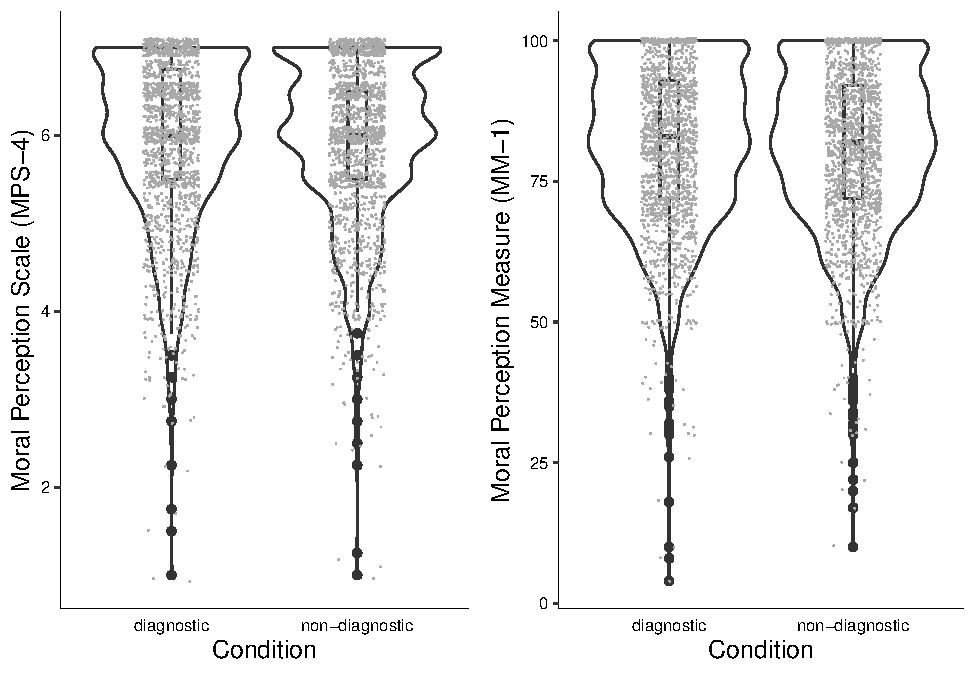
\includegraphics{moral_dilution_in_chunks_files/figure-latex/S4bothconditionplot-1.pdf}
\caption{\label{fig:S4bothconditionplot}Study 2: Differences in moral perception depending on condition}
\end{figure}

We conducted a linear-mixed-effects model to test if condition influenced MM-1 responses. Our outcome measure was MM-1, our predictor variable was condition; we allowed intercepts and the effect of condition to vary across participants. Overall, the model significantly predicted participants responses, and provided a better fit for the data than the baseline model, \(\chi\)\textsuperscript{2}(8) = 40.10, \emph{p} \textless{} .001. Condition significantly influenced MM-1 responses \emph{F}(1, 864) = 4.79, \emph{p} = .029, and was a significant predictor in the model \(b\) = 0.29, \emph{t}(864) = 2.19, \emph{p} = .029, see Figure~\ref{fig:S4bothconditionplot}.

In the supplementary analyses we report the effect of condition on moral perception for each description individually.

\hypertarget{study-5---good-and-bad-characters}{%
\section{Study 5 - Good and Bad Characters}\label{study-5---good-and-bad-characters}}

Studies 1-4 showed some evidence for the presence of the moral dilution effect. The effect appears to vary depending on specific factors. One factor we identified is the presence, and valence, of other descriptions. The dilution effect is observed for \emph{bad} characters when participants are presented with only \emph{bad} characters (Study 1). However this effect for \emph{bad} characters is less reliably observed (depending on the measure) when participants are additionally presented with descriptions of \emph{good} characters (Study 3). The reverse appears to be the case for \emph{good} characters, such that when \emph{good} characters are presented along with descriptions of \emph{bad} characters, a moral dilution effect is observed (Study 3). However, when descriptions of \emph{bad} characters are not present the moral dilution effect is not observed (Study 2), or less reliably observed (depending on the measure, Study 4). The aim of Study 5 was to test for the moral dilution effect in both good and bad characters, while attempting to eliminate the confounding influence of the presence of other descriptions by adopting a between-subjects design.

\hypertarget{study-5-method}{%
\subsection{Study 5: Method}\label{study-5-method}}

\hypertarget{study-5-participants-and-design}{%
\subsubsection{Study 5: Participants and design}\label{study-5-participants-and-design}}

Study 5 was a 2 \(\times\) 2 between-subjects factorial design. As in Study 3, the first independent variable was condition with two levels, diagnostic and non-diagnostic. The second independent variable was valence of character description, with two levels morally good and morally bad. We used the same two dependent variables as in previous studies (MPS-4, \(\alpha\) = 0.97, and MM-1).

A total sample of 2126 (1107 female, 1004 male, 5 non-binary, 2 other; 8 prefer not to say, \emph{M}\textsubscript{age} = 38.79, min = 2, max = 1995, \emph{SD} = 45.07) started the survey. Participants were recruited from MTurk and paid \$0.10 for their participation.

Participants who failed both manipulation checks were removed (\emph{n} = 376), leaving a total sample of 1750 participants (219.75 female, 214.50 male, 0.25 other, 0.25 prefer not to say; \emph{M}\textsubscript{age} = 37.82, min = 2, max = 454, \emph{SD} = 15.78).

\hypertarget{study-5-procedure-and-materials}{%
\subsubsection{Study 5: Procedure and materials}\label{study-5-procedure-and-materials}}

The materials for Study 5 were the same as those used in Study 3. Participants were randomly presented with a single character description: \emph{Sam}, \emph{Robin} (\emph{good} characters), \emph{Francis} and \emph{Alex} (\emph{bad} characters), and were randomly assigned to the diagnostic condition (containing diagnostic information only), or the non-diagnostic condition (where the character description additionally included non-diagnostic information). Study 5 was not pre-registered however our predictions were the same as those for Study 3.

\hypertarget{study-5-results}{%
\subsection{Study 5: Results}\label{study-5-results}}

The means and standard deviations for MPS-4 for each scenario are as follows:
\emph{Sam} (good),
\emph{M}\textsubscript{MPS-4} = 6.13, \emph{SD}\textsubscript{MPS-4} = 0.87,
\emph{Francis} (bad),
\emph{M}\textsubscript{MPS-4} = 3.72, \emph{SD}\textsubscript{MPS-4} = 2.16,
\emph{Alex} (bad),
\emph{M}\textsubscript{MPS-4} = 3.73, \emph{SD}\textsubscript{MPS-4} = 2.08,
\emph{Robin} (good),
\emph{M}\textsubscript{MPS-4} = 6.19, \emph{SD}\textsubscript{MPS-4} = 0.85. There was significant variation depending on the description, \emph{F}(3,1746) = 333.96, \emph{p} \textless{} .001, partial \(\eta\)\textsuperscript{2} = 0.36. Both the \emph{good} characters (\emph{Robin} and \emph{Sam}) were rated significantly more favorably than both the \emph{bad} characters (\emph{Alex} and \emph{Francis}; all \emph{p}s \textless{} .001). There were no differences between \emph{Robin} and \emph{Sam} (\emph{good}: \emph{p} = .938) or between \emph{Alex} and \emph{Francis} (\emph{bad}; (\emph{p} \textgreater{} .999)).

The means and standard deviations for MM-1 for each scenario are as follows:
\emph{Sam} (good),
\emph{M}\textsubscript{MM-1} = 84.52, \emph{SD}\textsubscript{MM-1} = 15.49;
\emph{Francis} (bad),
\emph{M}\textsubscript{MM-1} = 44.51, \emph{SD}\textsubscript{MM-1} = 35.08;
\emph{Alex} (bad),
\emph{M}\textsubscript{MM-1} = 45.85, \emph{SD}\textsubscript{MM-1} = 34.36;
\emph{Robin} (good),
\emph{M}\textsubscript{MM-1} = 85.15, \emph{SD}\textsubscript{MM-1} = 14.61. There was significant variation depending on the description, \emph{F}(3,1746) = 324.34, \emph{p} \textless{} .001, partial \(\eta\)\textsuperscript{2} = 0.36. Both the \emph{good} characters (\emph{Robin} and \emph{Sam}) were rated significantly more favorably than both the \emph{bad} characters (\emph{Alex} and \emph{Francis}; all \emph{p}s \textless{} .001). There were no differences between \emph{Robin} and \emph{Sam} (\emph{good}: \emph{p} = .985) or between \emph{Alex} and \emph{Francis} (\emph{bad}; (\emph{p} = .882)).

\hypertarget{testing-for-the-interaction}{%
\subsubsection{Testing for the Interaction}\label{testing-for-the-interaction}}

We conducted a 2 \(\times\) 2 between subjects ANOVA to test for an interaction between valence and condition.
As expected, on its own, condition did not influence responses to the MPS-4
, \emph{F}(1, 1746) = 0.01, \emph{p} = .907
; valence significantly predicted responses,
, \emph{F}(1, 1746) = 1,004.46, \emph{p} \textless{} .001
; and there was a significant condition \(\times\) valence interaction,
, \emph{F}(1, 1746) = 5.45, \emph{p} = .020.

We conducted a 2 \(\times\) 2 between subjects ANOVA to test for an interaction between valence and condition.
As expected, on its own, condition did not influence responses to the MPS-4
, \emph{F}(1, 1746) = 0.21, \emph{p} = .650
; valence significantly predicted responses,
, \emph{F}(1, 1746) = 977.37, \emph{p} \textless{} .001
; and there was a significant condition \(\times\) valence interaction,
, \emph{F}(1, 1746) = 9.63, \emph{p} = .002.

\hypertarget{differences-in-the-bad-descriptions-1}{%
\subsection{\texorpdfstring{Differences in the \emph{Bad} Descriptions}{Differences in the Bad Descriptions}}\label{differences-in-the-bad-descriptions-1}}

To interpret the interaction effect, we conducted separate analyses for the Good and Bad descriptions.

For the \emph{bad} characters, there was no significant difference in responses to MPS-4 between the diagnostic condition (\emph{M} = 3.63, \emph{SD} = 2.21) and the non-diagnostic condition (\emph{M} = 3.81, \emph{SD} = 2.03) depending on condition, \emph{t}(834.36) = -1.23, \emph{p} = .221, \emph{d} = 0.08.

For the \emph{bad} characters, there was no significant difference in responses to MPS-4 between the diagnostic condition (\emph{M} = 43.35, \emph{SD} = 35.56) and the non-diagnostic condition (\emph{M} = 46.86, \emph{SD} = 33.85) depending on condition, \emph{t}(843.09) = -1.48, \emph{p} = .140, \emph{d} = 0.10.

\hypertarget{differences-in-the-good-descriptions-1}{%
\subsection{\texorpdfstring{Differences in the \emph{Good} Descriptions}{Differences in the Good Descriptions}}\label{differences-in-the-good-descriptions-1}}

For the \emph{good} characters, there was no significant difference in responses to MPS-4 between the diagnostic condition (\emph{M} = 6.25, \emph{SD} = 0.84) and the non-diagnostic condition (\emph{M} = 6.07, \emph{SD} = 0.87) depending on condition, \emph{t}(886.55) = 3.16, \emph{p} = .002, \emph{d} = 0.21.

For the \emph{good} characters, there was no significant difference in responses to MPS-4 between the diagnostic condition (\emph{M} = 87.11, \emph{SD} = 13.75) and the non-diagnostic condition (\emph{M} = 82.74, \emph{SD} = 15.89) depending on condition, \emph{t}(883.93) = 4.40, \emph{p} \textless{} .001, \emph{d} = 0.29.

\begin{figure}
\centering
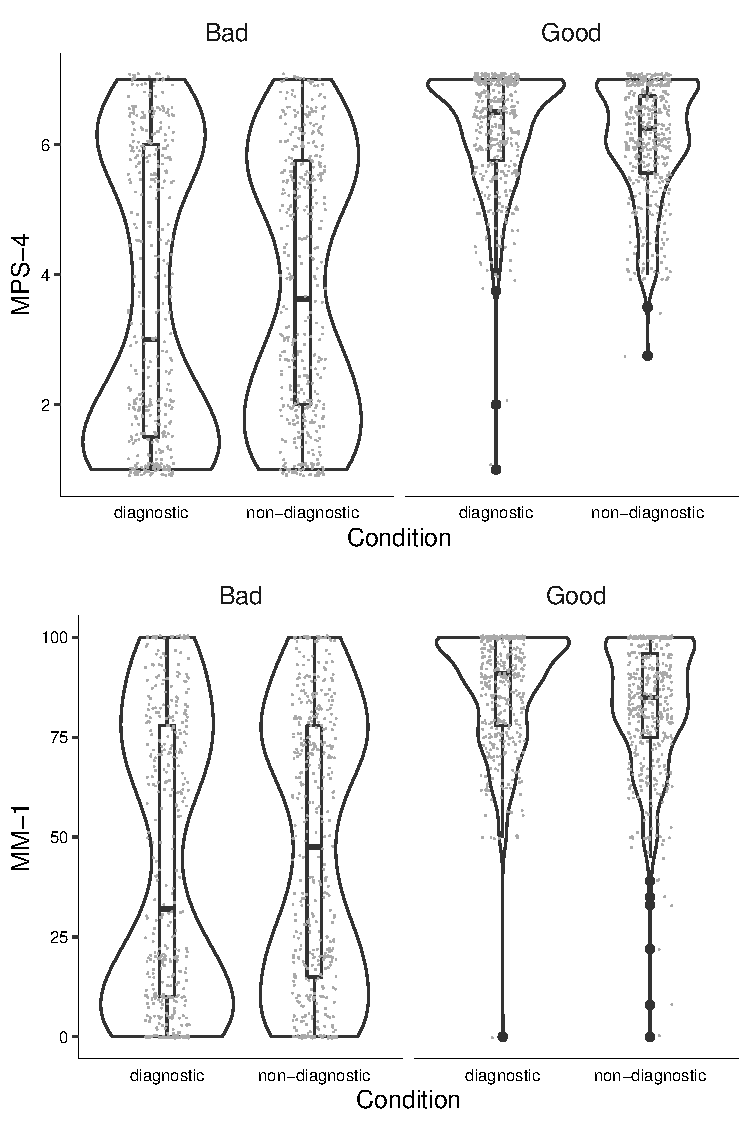
\includegraphics{moral_dilution_in_chunks_files/figure-latex/S5bothconditionplot-1.pdf}
\caption{\label{fig:S5bothconditionplot}Study 3: Differences in moral perception depending on condition}
\end{figure}

In the supplementary analyses we report the effect of condition on moral perception for each description individually.

\newpage

\hypertarget{discussion}{%
\section{Discussion}\label{discussion}}

\hypertarget{accessibility-statement}{%
\section{Accessibility Statement}\label{accessibility-statement}}

All data and analysis code are publicly available on this project's OSF page at \color{blue}\url{https://osf.io/mdnpv/?view_only=77883e3fbc3d45f1a35fe92d5318cb67}\color{black}.

\newpage

\hypertarget{references}{%
\section*{References}\label{references}}
\addcontentsline{toc}{section}{References}

\hypertarget{refs}{}
\leavevmode\hypertarget{ref-grizzard_validating_2020}{}%
Grizzard, M., Fitzgerald, K., Francemone, C. J., Ahn, C., Huang, J., Walton, J., \ldots{} Eden, A. (2020). Validating the extended character morality questionnaire. \emph{Media Psychology}, \emph{23}(1), 107--130. \url{https://doi.org/10.1080/15213269.2019.1572523}

\leavevmode\hypertarget{ref-mchugh_moral_2022}{}%
McHugh, C., McGann, M., Igou, E. R., \& Kinsella, E. L. (2022). Moral Judgment as Categorization (MJAC). \emph{Perspectives on Psychological Science}, \emph{17}(1), 131--152. \url{https://doi.org/10.1177/1745691621990636}

\leavevmode\hypertarget{ref-schein_theory_2018}{}%
Schein, C., \& Gray, K. J. (2018). The Theory of Dyadic Morality: Reinventing Moral Judgment by Redefining Harm. \emph{Personality and Social Psychology Review}, \emph{22}(1), 32--70. \url{https://doi.org/10.1177/1088868317698288}

\leavevmode\hypertarget{ref-walker_better_2021}{}%
Walker, A. C., Turpin, M. H., Fugelsang, J. A., \& Białek, M. (2021). Better the two devils you know, than the one you don't: Predictability influences moral judgments of immoral actors. \emph{Journal of Experimental Social Psychology}, \emph{97}, 104220. \url{https://doi.org/10.1016/j.jesp.2021.104220}


\end{document}
